% Figure 5 of "Galashin's Conjecture 4.3 via a convex gradient": two winding-one partitions.
% Source of the figure, typeset in the paper's own fonts (T1, Latin Modern, 11pt) at the paper's text
% width (6.5in), so \includegraphics does not rescale it. Illustrates CLH-5; it adds no assertion.
% Every value drawn is read from these Lean output lines:
%   EX02 window(1-based)=[3, 5, 1, 2, 4] n=5 modulus=25 rank=3 coloops=[]
%   EX02 s_x (x=1..n)=[3, 4, 1, 5, 2]
%   EX02 exitPos(x=1..n)=[1, 6, 11, 16, 21]
%   EX02 entryPos(x=1..n, entry of strand into x)=[14, 19, 4, 24, 9]
%   EX02 crossEdges(paper labels)=[(1, 2), (2, 3), (2, 4), (3, 5), (4, 5), (5, 1), (5, 2)]
%   EX02 crossEdges with s_p=q (paper labels)=[(2, 4), (4, 5), (5, 2)]
%   EX03 partition A {(1,2,3,5),(2,4,5)}: windings=[5, 5] (n=5) lengths=[4, 3] edge multiset = crossEdges: true
%   EX03 partition B {(1,2,4,5),(2,3,5)}: windings=[5, 5] (n=5) lengths=[4, 3] edge multiset = crossEdges: true
% Build: pdflatex <this file> && pdftocairo -svg <this file>.pdf <this file>.svg
\documentclass[11pt]{standalone}
\usepackage[T1]{fontenc}
\usepackage{lmodern}
\usepackage{amsmath,amssymb}
\usepackage{tikz}
\usetikzlibrary{arrows.meta,positioning,calc}

% the palette of the paper's other figures: blue solid for the first strand or arc, ochre dashed for the second
\definecolor{ink}{HTML}{233740}
\definecolor{muted}{HTML}{65757D}
\definecolor{pblue}{HTML}{0072B2}
\definecolor{qochre}{HTML}{B87827}

\tikzset{
  base/.style={draw=muted, line width=0.5pt},
  exit/.style={circle, draw=ink, fill=white, line width=0.6pt, inner sep=0pt, minimum size=4.6pt},
  entry/.style={circle, draw=ink, fill=ink, line width=0.6pt, inner sep=0pt, minimum size=4.6pt},
  exitP/.style={exit, draw=pblue}, entryP/.style={entry, draw=pblue, fill=pblue},
  exitQ/.style={exit, draw=qochre}, entryQ/.style={entry, draw=qochre, fill=qochre},
  strandP/.style={pblue, line width=1.1pt, -{Stealth[length=5pt,width=4.2pt]}, shorten >=2.4pt},
  strandQ/.style={qochre, line width=1.1pt, dash pattern=on 4pt off 1.6pt, -{Stealth[length=5pt,width=4.2pt]}, shorten >=2.4pt},
  lab/.style={font=\footnotesize, inner sep=1.2pt, text=ink},
  labm/.style={font=\small, inner sep=1.2pt, text=ink},
  labP/.style={font=\small, inner sep=1.2pt, text=pblue},
  labQ/.style={font=\small, inner sep=1.2pt, text=qochre},
  muted text/.style={text=muted},
  ttl/.style={font=\small, text=ink, inner sep=0pt},
  negE/.style={font=\small, text=pblue, inner sep=0pt},
  posE/.style={font=\small, text=qochre, inner sep=0pt},
  zeroE/.style={font=\small, text=ink, inner sep=0pt},
  idx/.style={font=\footnotesize, text=muted, inner sep=0pt},
}
\tikzset{
  vtx/.style={circle, draw=ink, fill=white, line width=0.6pt, inner sep=0pt, minimum size=0.62cm, font=\small, text=ink},
  cycP/.style={pblue, line width=1.1pt, -{Stealth[length=5pt,width=4.2pt]}, shorten >=1pt, shorten <=1pt},
  cycQ/.style={qochre, line width=1.1pt, dash pattern=on 4pt off 1.6pt, -{Stealth[length=5pt,width=4.2pt]}, shorten >=1pt, shorten <=1pt},
  labmP/.style={font=\small, text=pblue, inner sep=1.2pt}, labmQ/.style={font=\small, text=qochre, inner sep=1.2pt},
}

\begin{document}
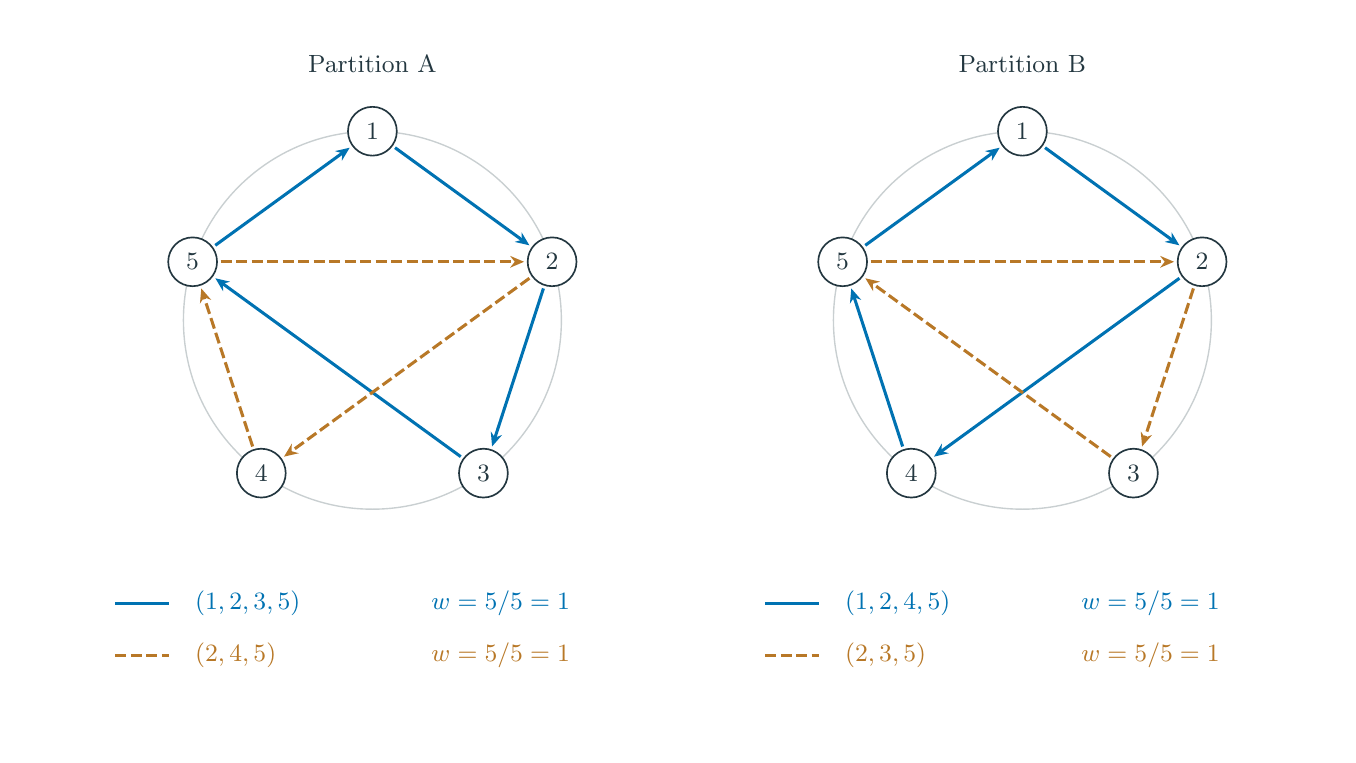
\begin{tikzpicture}[x=1cm,y=1cm]
\useasboundingbox (-0.25000,-8.61522) rectangle (16.26000,0.36522);
\node[ttl] at (4.128,-0.100) {Partition A}; %t title0
\draw[draw=muted!35, line width=0.5pt] (4.128,-3.350) circle (2.400); %o 0 5
\node[vtx] (v0_1) at (4.128,-0.950) {1}; %t 0-vertex1
\node[vtx] (v0_2) at (6.410,-2.608) {2}; %t 0-vertex2
\node[vtx] (v0_3) at (5.538,-5.292) {3}; %t 0-vertex3
\node[vtx] (v0_4) at (2.717,-5.292) {4}; %t 0-vertex4
\node[vtx] (v0_5) at (1.845,-2.608) {5}; %t 0-vertex5
\draw[cycP] (v0_1) -- (v0_2); %c 0-0 1,2
\draw[cycP] (v0_2) -- (v0_3); %c 0-0 2,3
\draw[cycP] (v0_3) -- (v0_5); %c 0-0 3,5
\draw[cycP] (v0_5) -- (v0_1); %c 0-0 5,1
\draw[cycP, -] (0.828,-6.950) -- (1.578,-6.950); %k 0-0
\node[labmP, anchor=west] at (1.828,-6.950) {$(1,2,3,5)$}; %t 0-cycle0
\node[labmP, anchor=west] at (4.828,-6.950) {$w=5/5=1$}; %t 0-wind0
\draw[cycQ] (v0_2) -- (v0_4); %c 0-1 2,4
\draw[cycQ] (v0_4) -- (v0_5); %c 0-1 4,5
\draw[cycQ] (v0_5) -- (v0_2); %c 0-1 5,2
\draw[cycQ, -] (0.828,-7.610) -- (1.578,-7.610); %k 0-1
\node[labmQ, anchor=west] at (1.828,-7.610) {$(2,4,5)$}; %t 0-cycle1
\node[labmQ, anchor=west] at (4.828,-7.610) {$w=5/5=1$}; %t 0-wind1
\node[ttl] at (12.383,-0.100) {Partition B}; %t title1
\draw[draw=muted!35, line width=0.5pt] (12.383,-3.350) circle (2.400); %o 1 5
\node[vtx] (v1_1) at (12.383,-0.950) {1}; %t 1-vertex1
\node[vtx] (v1_2) at (14.665,-2.608) {2}; %t 1-vertex2
\node[vtx] (v1_3) at (13.793,-5.292) {3}; %t 1-vertex3
\node[vtx] (v1_4) at (10.972,-5.292) {4}; %t 1-vertex4
\node[vtx] (v1_5) at (10.100,-2.608) {5}; %t 1-vertex5
\draw[cycP] (v1_1) -- (v1_2); %c 1-0 1,2
\draw[cycP] (v1_2) -- (v1_4); %c 1-0 2,4
\draw[cycP] (v1_4) -- (v1_5); %c 1-0 4,5
\draw[cycP] (v1_5) -- (v1_1); %c 1-0 5,1
\draw[cycP, -] (9.082,-6.950) -- (9.832,-6.950); %k 1-0
\node[labmP, anchor=west] at (10.082,-6.950) {$(1,2,4,5)$}; %t 1-cycle0
\node[labmP, anchor=west] at (13.082,-6.950) {$w=5/5=1$}; %t 1-wind0
\draw[cycQ] (v1_2) -- (v1_3); %c 1-1 2,3
\draw[cycQ] (v1_3) -- (v1_5); %c 1-1 3,5
\draw[cycQ] (v1_5) -- (v1_2); %c 1-1 5,2
\draw[cycQ, -] (9.082,-7.610) -- (9.832,-7.610); %k 1-1
\node[labmQ, anchor=west] at (10.082,-7.610) {$(2,3,5)$}; %t 1-cycle1
\node[labmQ, anchor=west] at (13.082,-7.610) {$w=5/5=1$}; %t 1-wind1
\end{tikzpicture}
\end{document}
